<<<<<<< HEAD
\section{Punto de Vista de Proceso de Negocio}

El punto de vista de la cooperación de los procesos comerciales se utiliza para mostrar las relaciones de uno o más procesos comerciales entre sí y/o con su entorno. Puede utilizarse tanto para crear un diseño de alto nivel de los procesos empresariales dentro de su contexto como para proporcionar a un director operacional responsable de uno o más de esos procesos una visión de sus dependencias. Los aspectos importantes de la cooperación en los procesos empresariales son:

\begin{itemize}
	\item Relaciones causales entre los principales procesos comerciales de la empresa
	\item Mapeo de los procesos comerciales en las funciones comerciales
	\item Realización de servicios por procesos comerciales
	\item Uso de datos compartidos
\end{itemize}

Cada una de ellas puede considerarse un "subpunto de vista" del punto de vista de la cooperación en los procesos comerciales.

\subsection{Modelo de Proceso de Negocio}
\begin{figure}[h!]
	\centering
	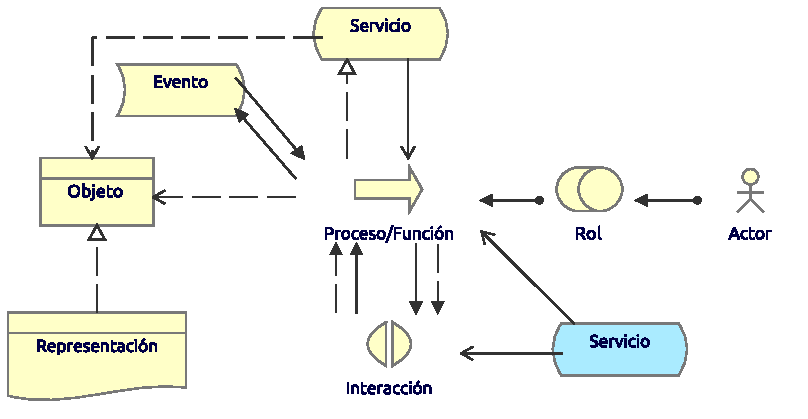
\includegraphics[width=.8\linewidth]{imgs/modelo/ProcesoNegocio}
	\caption{Modelo Proceso de Negocio}
\end{figure}

Un proceso empresarial representa una secuencia de comportamientos empresariales que logra un resultado específico, como un conjunto definido de productos o servicios empresariales.
Un proceso de negocios describe el comportamiento interno realizado por un rol de negocios que se requiere para producir un conjunto de productos y servicios. Para un consumidor, los productos y servicios son relevantes y el comportamiento requerido es meramente una caja negra, de ahí la designación "interno".
Un proceso comercial complejo puede ser una agregación de otros procesos de grano más fino. A cada uno de ellos se le pueden asignar funciones más finas.
Existe una relación potencial de muchos a muchos entre los procesos de negocios y las funciones de negocios. En términos informales, los procesos describen algún tipo de "flujo" de actividades, mientras que las funciones agrupan las actividades según las aptitudes, los conocimientos, los recursos, etc. requeridos. Un proceso empresarial puede ser desencadenado por, o desencadenar, cualquier otro elemento de comportamiento empresarial (por ejemplo, un acto empresarial, un proceso empresarial, una función empresarial o una interacción empresarial). Un proceso empresarial puede acceder a objetos empresariales. Un proceso empresarial puede realizar uno o más servicios empresariales y pueden utilizar servicios comerciales (internos) o servicios de aplicación. Se puede asignar una función empresarial a un proceso empresarial para realizar este proceso manualmente. Un proceso empresarial automatizado puede realizarse mediante un proceso de aplicación. El nombre de un proceso empresarial debe indicar claramente una secuencia predefinida de acciones, y puede incluir la palabra "proceso". Ejemplos de ello son "adjudicar la reclamación", "incorporación de empleados", "proceso de aprobación" o "presentación de informes financieros". \\

Un objeto comercial representa un concepto utilizado dentro de un dominio comercial determinado. Un contrato representa una especificación formal o informal de un acuerdo entre un proveedor y un consumidor en el que se especifican los derechos y obligaciones asociados a un producto y se establecen parámetros funcionales y no funcionales para la interacción. Una representación representa una forma perceptible de la información que lleva un objeto comercial.

\clearpage
\subsection{Caso  de Proceso de Negocio}
\begin{figure}[h!]
	\centering
	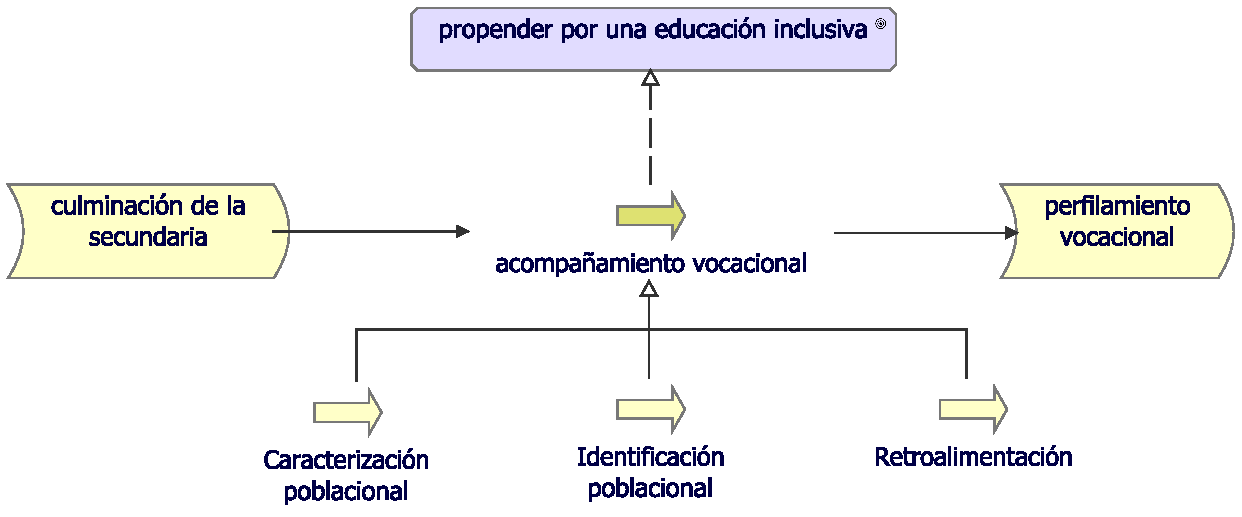
\includegraphics[width=.9\linewidth]{imgs/caso/negocio/proceso}
	\caption{Caso Proceso de Negocio}
\end{figure}

Después de efectuar una revisión documental sobre los procesos del MEN dispuestos para dar alcance a uno de sus principales objetivos, propender por una educación inclusiva, desde nuestra organización proponemos la inclusión de un nuevo proceso capaz de fortalecer y afianzar en la sociedad, ese objetivo de carácter político que conlleve a una educación inclusiva eficiente en cuanto al desarrollo personal y profesional de la comunidad se refiere. Asimismo, este proceso novedoso en el marco actual de la organización, se especializa en tres procesos de carácter secuencial dispuestos de la siguiente manera, una caracterización poblacional, una Identificación poblacional posterior, y finalmente, una retroalimentación individualizada para cada estudiante que culmina la secundaria, evento inicial de nuestro proceso de acompañamiento vocacional, el cual culmina con el perfilamiento vocacional de cada uno de estos estudiantes.
=======
\section{Punto de Vista de Proceso de Negocio}

El punto de vista del proceso de negocio, es en donde se definen los procesos organizacionales del proyecto, es decir, lo que se convertirá en el paradigma alrededor del cual la organización resuelve toda su misión, sus funciones, objetivos. En concreto es el Core en donde se determina la funcionalidad organizacional.
Este punto de vista contribuye al entendimiento real de lo que se requiere con el proyecto, es decir, su objetivo organizaciones, todo desde un punto de vista administrativo, dando una visión más amplia y completa a lo que se refiere con la finalidad del proyecto.

\subsection{Modelo de Proceso de Negocio}
\begin{figure}[h!]
	\centering
	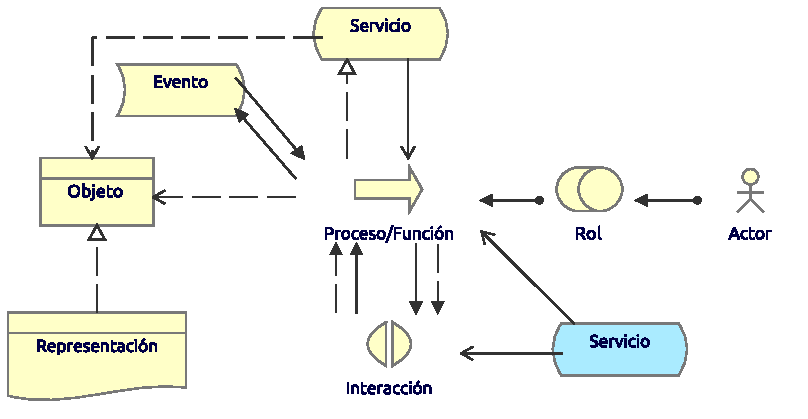
\includegraphics[width=.8\linewidth]{imgs/modelo/ProcesoNegocio}
	\caption{Modelo Proceso de Negocio}
\end{figure}

El modelo para el punto de vista de proceso de negocio, se centra en un proceso o función que como su nombre lo indica es el desarrollo del objetivo qu se requiere, asimismo cuenta con una serie de eventos de negocio los cuales anteceden y preceden al proceso de negocio, de la misma manera, está conformado por servicios, objetos y representaciones, además de definir el rol del proceso y el actor que interviene en el mismo.

\clearpage
\subsection{Caso  de Proceso de Negocio}
\begin{figure}[h!]
	\centering
	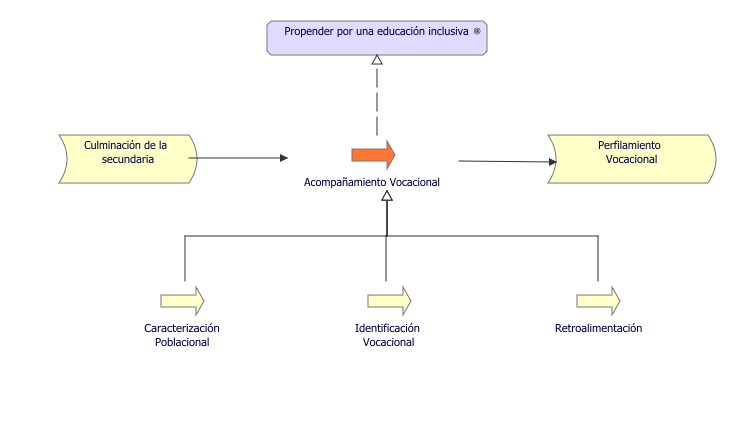
\includegraphics[width=.9\linewidth]{imgs/caso/negocio/ProcesoNegocio}
	\caption{Caso Proceso de Negocio}
\end{figure}

En el caso de nuestro proyecto, el proceso principal es el acompañamiento vocacional, vinculado al gran objetivo de propender por una educación inclusiva y dos eventos de negocio muy importantes que anteceden y preceden al proceso de negocio, el evento que antecede a este proceso de negocio es la culminación de la secundaria, posteriormente interviene el proceso de negocio con el acompañamiento vocacional y precede a este el evento de negocio del perfilamiento vocacional como finalización a este proceso, además este proceso principal está acompañado de tres subprocesos que en orden correspondiente son, en primer lugar la caracterización poblacional, continua con la identificación vocacional y finaliza con una retroalimentación.
>>>>>>> 15cbc3c11dec80c922f55a4b597d60cfea83963c
